\chapter{使用说明}

本章对论文模板中已预定义的常用环境和排版方式进行说明,并通过示例展示其具体用法。作者在撰写论文过程中,可参考本章内容正确使用定义、公式、定理、图表、算法以及引用等环境,从而保证论文结构清晰、格式统一,符合学位论文排版规范。

\section{问题定义}

在论文研究中,问题描述、模型假设以及符号约定等内容通常需要以明确、规范的方式给出。为此,本模板提供了“定义(Definition)”环境,用于描述概念、变量或研究对象。

定义环境具有自动编号功能,定义标题采用加粗形式,定义内容采用正文字体排版,适合用于形式化描述研究问题。

\begin{definition}[示例定义]
设……则……
\end{definition}

在实际写作中,作者可在定义标题中给出简要说明,也可省略标题,仅保留“定义 + 编号”的形式。

\section{公式}

数学公式是论文中表达模型与理论的重要手段。模板中推荐使用 \texttt{equation} 环境排版带编号公式,以便在正文中进行交叉引用。示例如下:

\subsection{带编号的公式}

\begin{equation}
  f(x)=\frac{a^\top x + b}{c^\top x + d}.
\end{equation}

\subsection{不带编号的公式}

\begin{equation}
\notag
   f(x)=\frac{a^\top x + b}{c^\top x + d}.
\end{equation}

\section{图表示例}

论文中的实验结果、结构示意或数据可视化内容通常通过图形进行展示。图像应使用 \texttt{figure} 环境插入,并配合图题与标签进行说明和引用。

单幅图像的使用示例如下:

\begin{figure}[htbp]
  \centering
  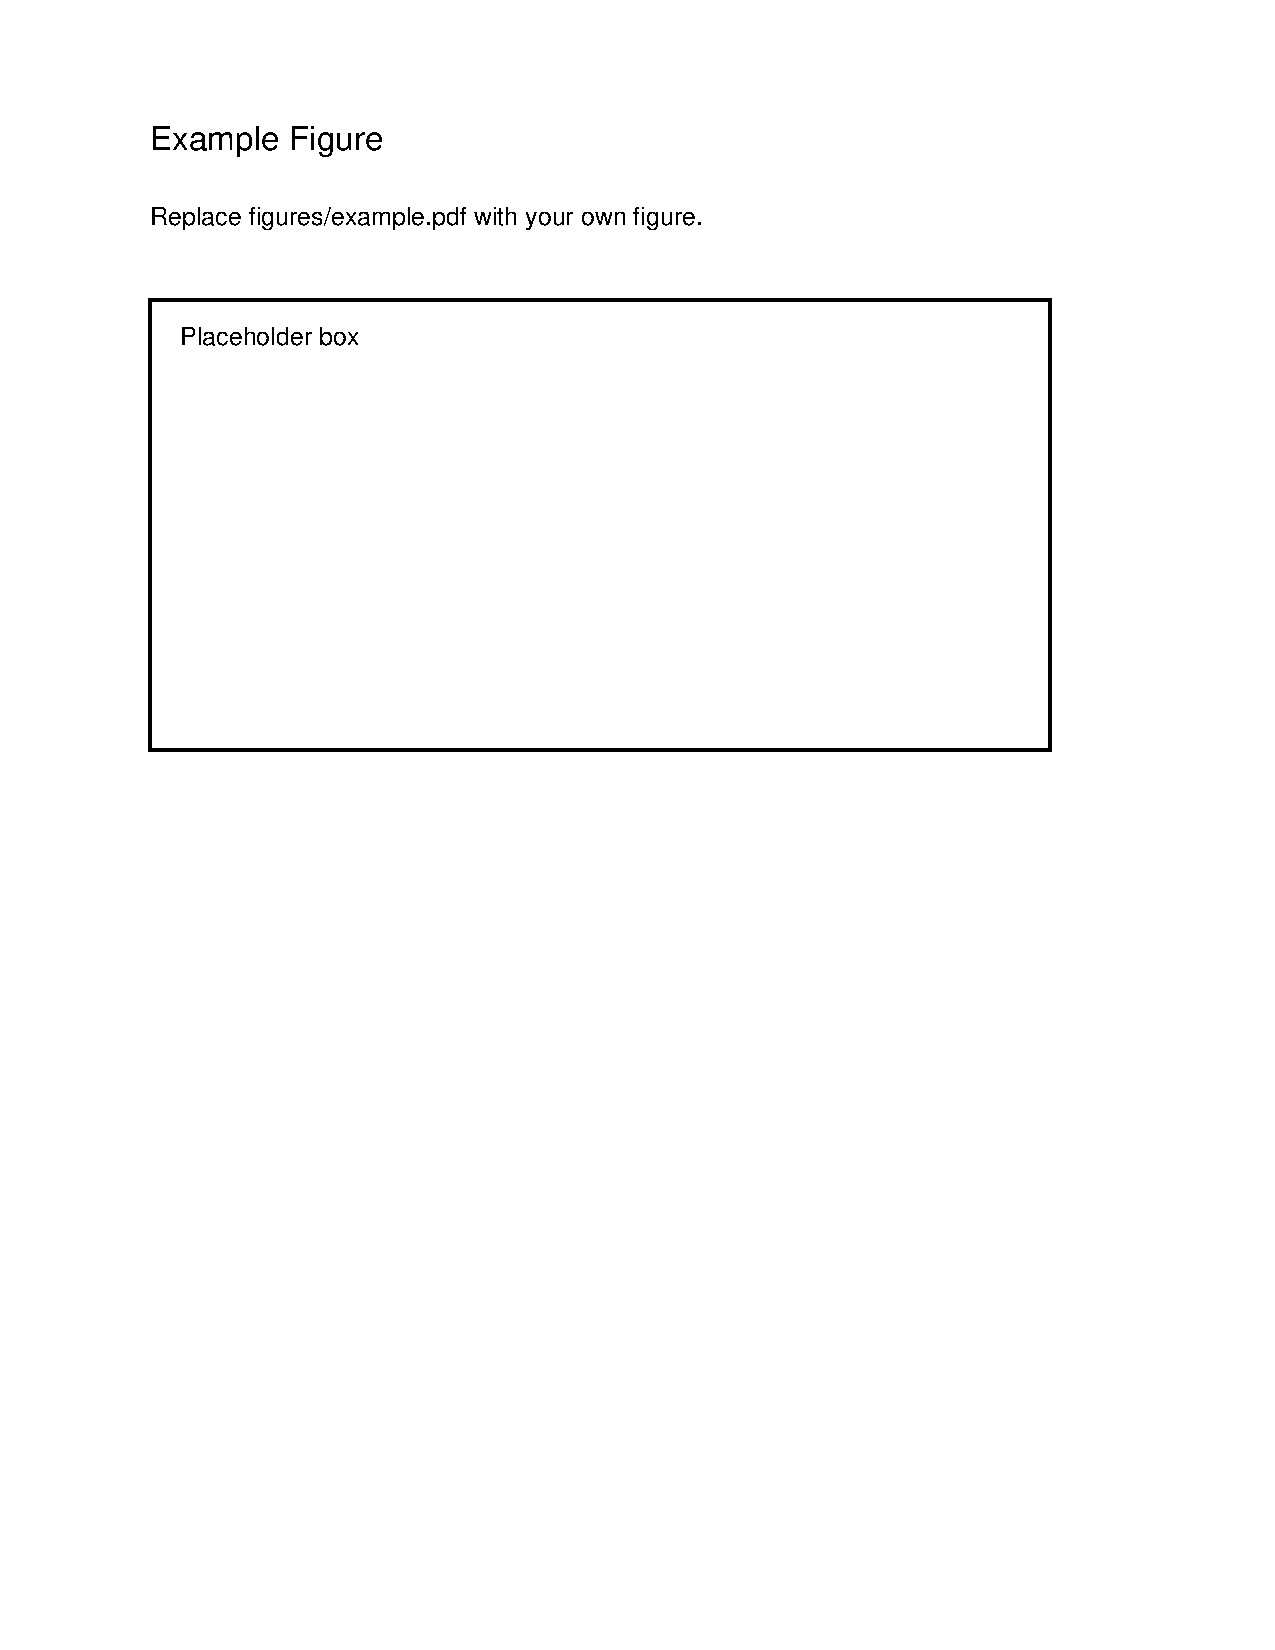
\includegraphics[width=0.65\linewidth]{figures/example.jpg}
  \caption{示例图}
  \label{fig:example}
\end{figure}

当需要展示多幅相关图像时,可采用并排或矩阵式排布方式,通过多次 \texttt{\textbackslash includegraphics} 命令实现。例如:

\begin{figure}[htbp]
  \begin{center}
    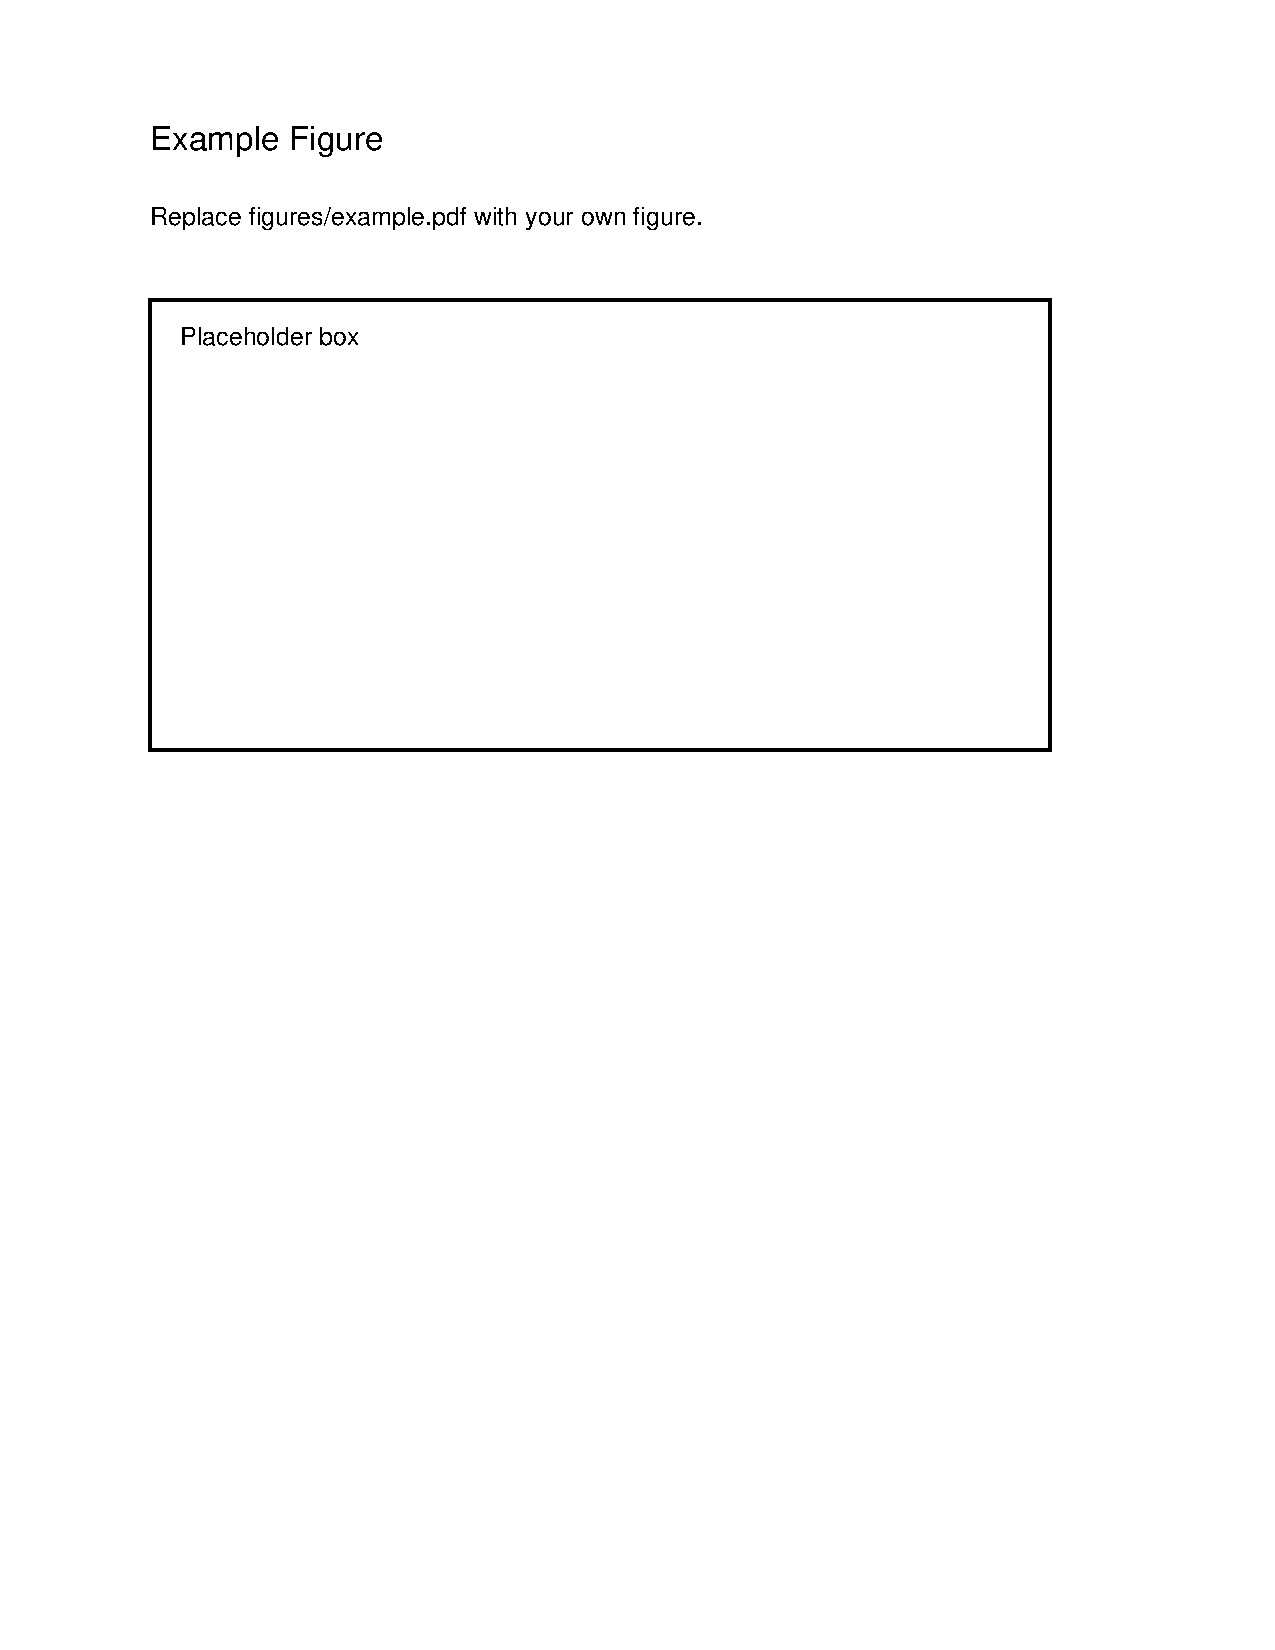
\includegraphics[width=0.45\linewidth]{figures/example.jpg}
    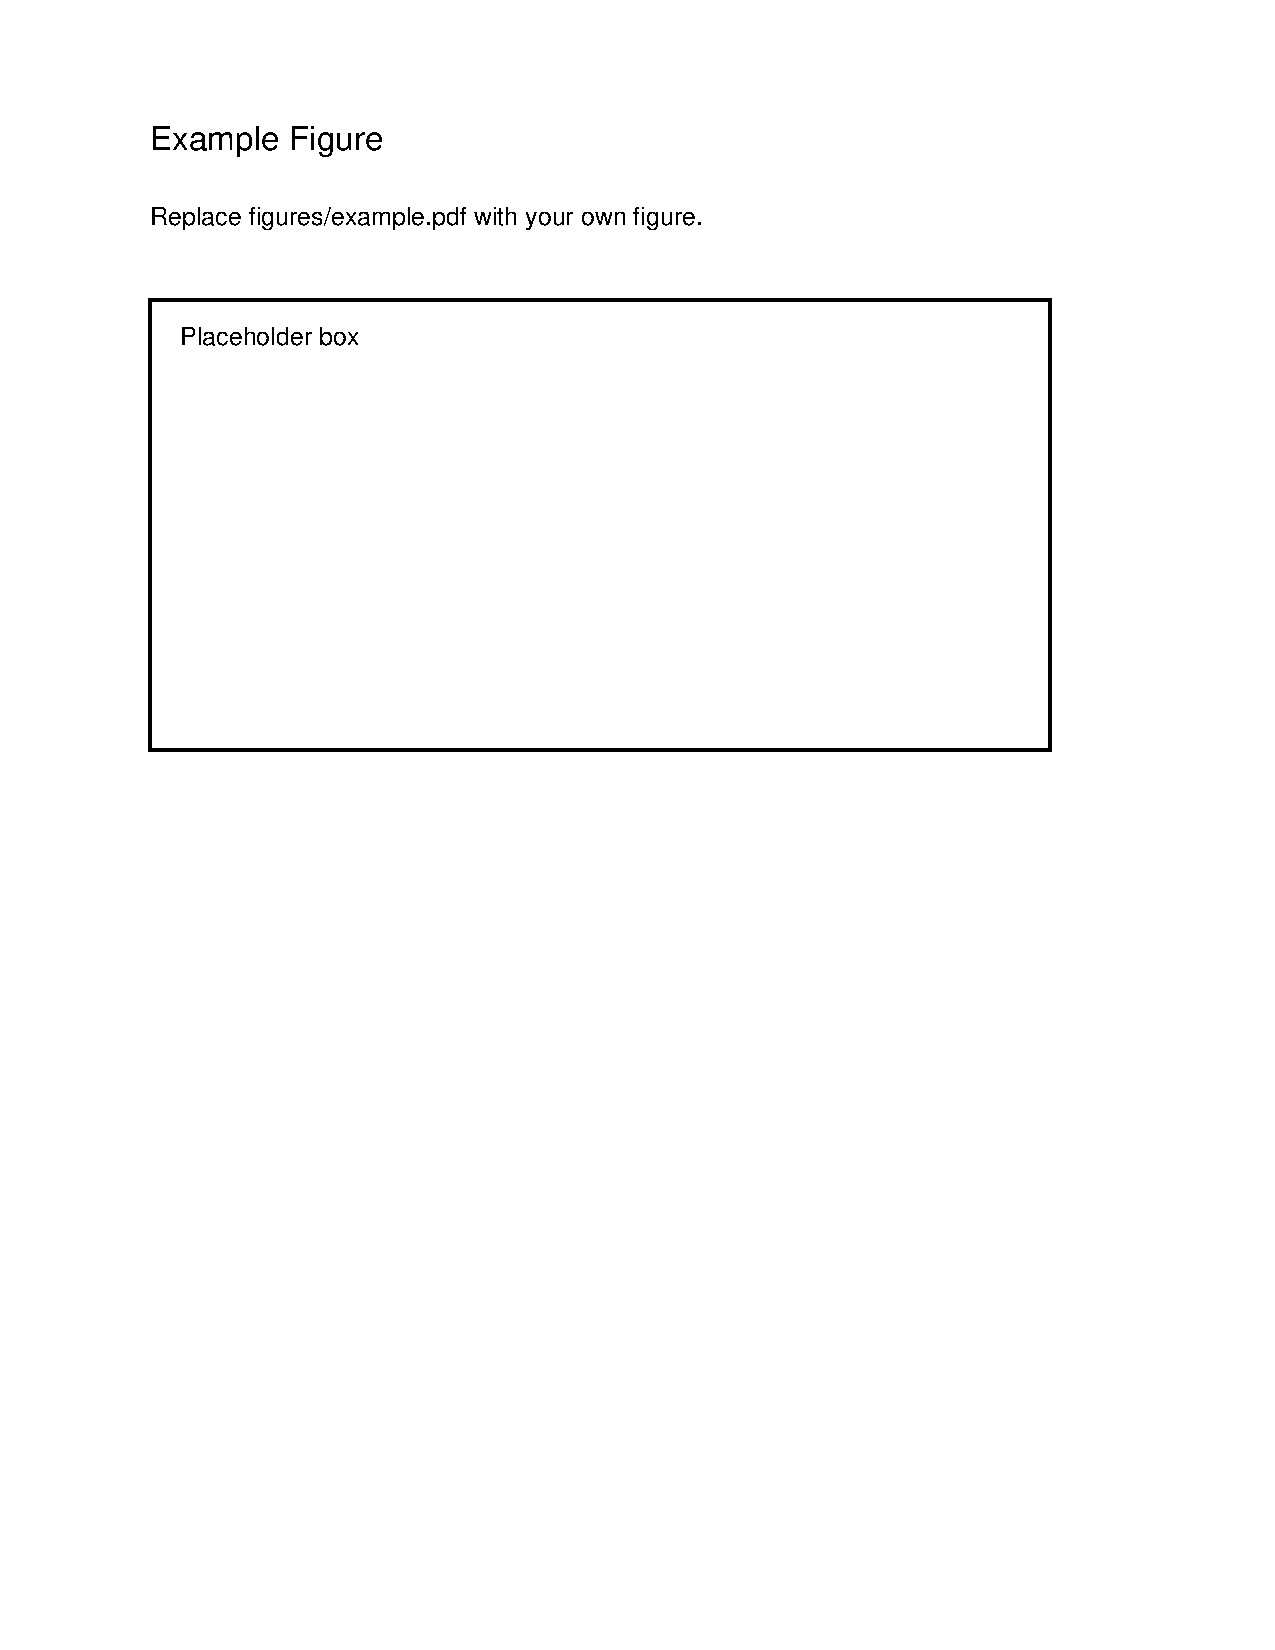
\includegraphics[width=0.45\linewidth]{figures/example.jpg}
  \end{center}
  \begin{center}
    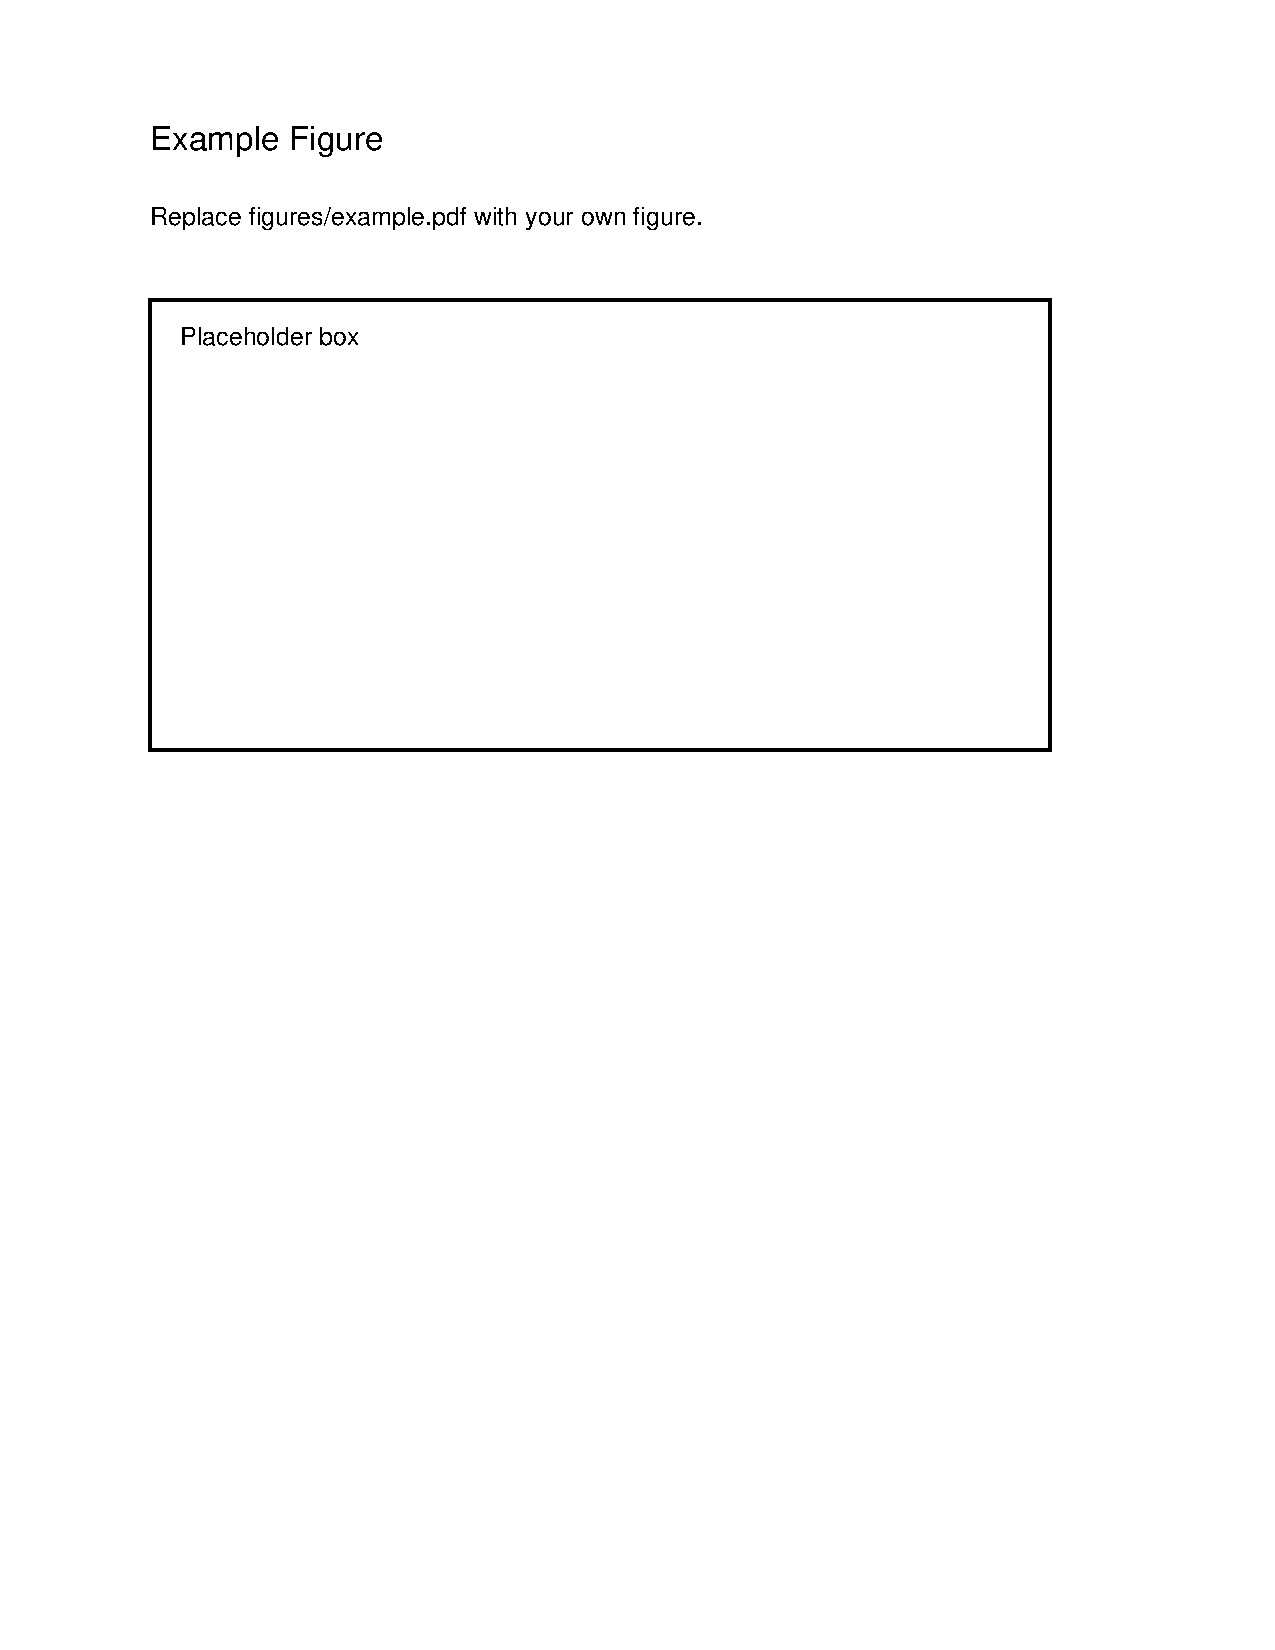
\includegraphics[width=0.45\linewidth]{figures/example.jpg}
    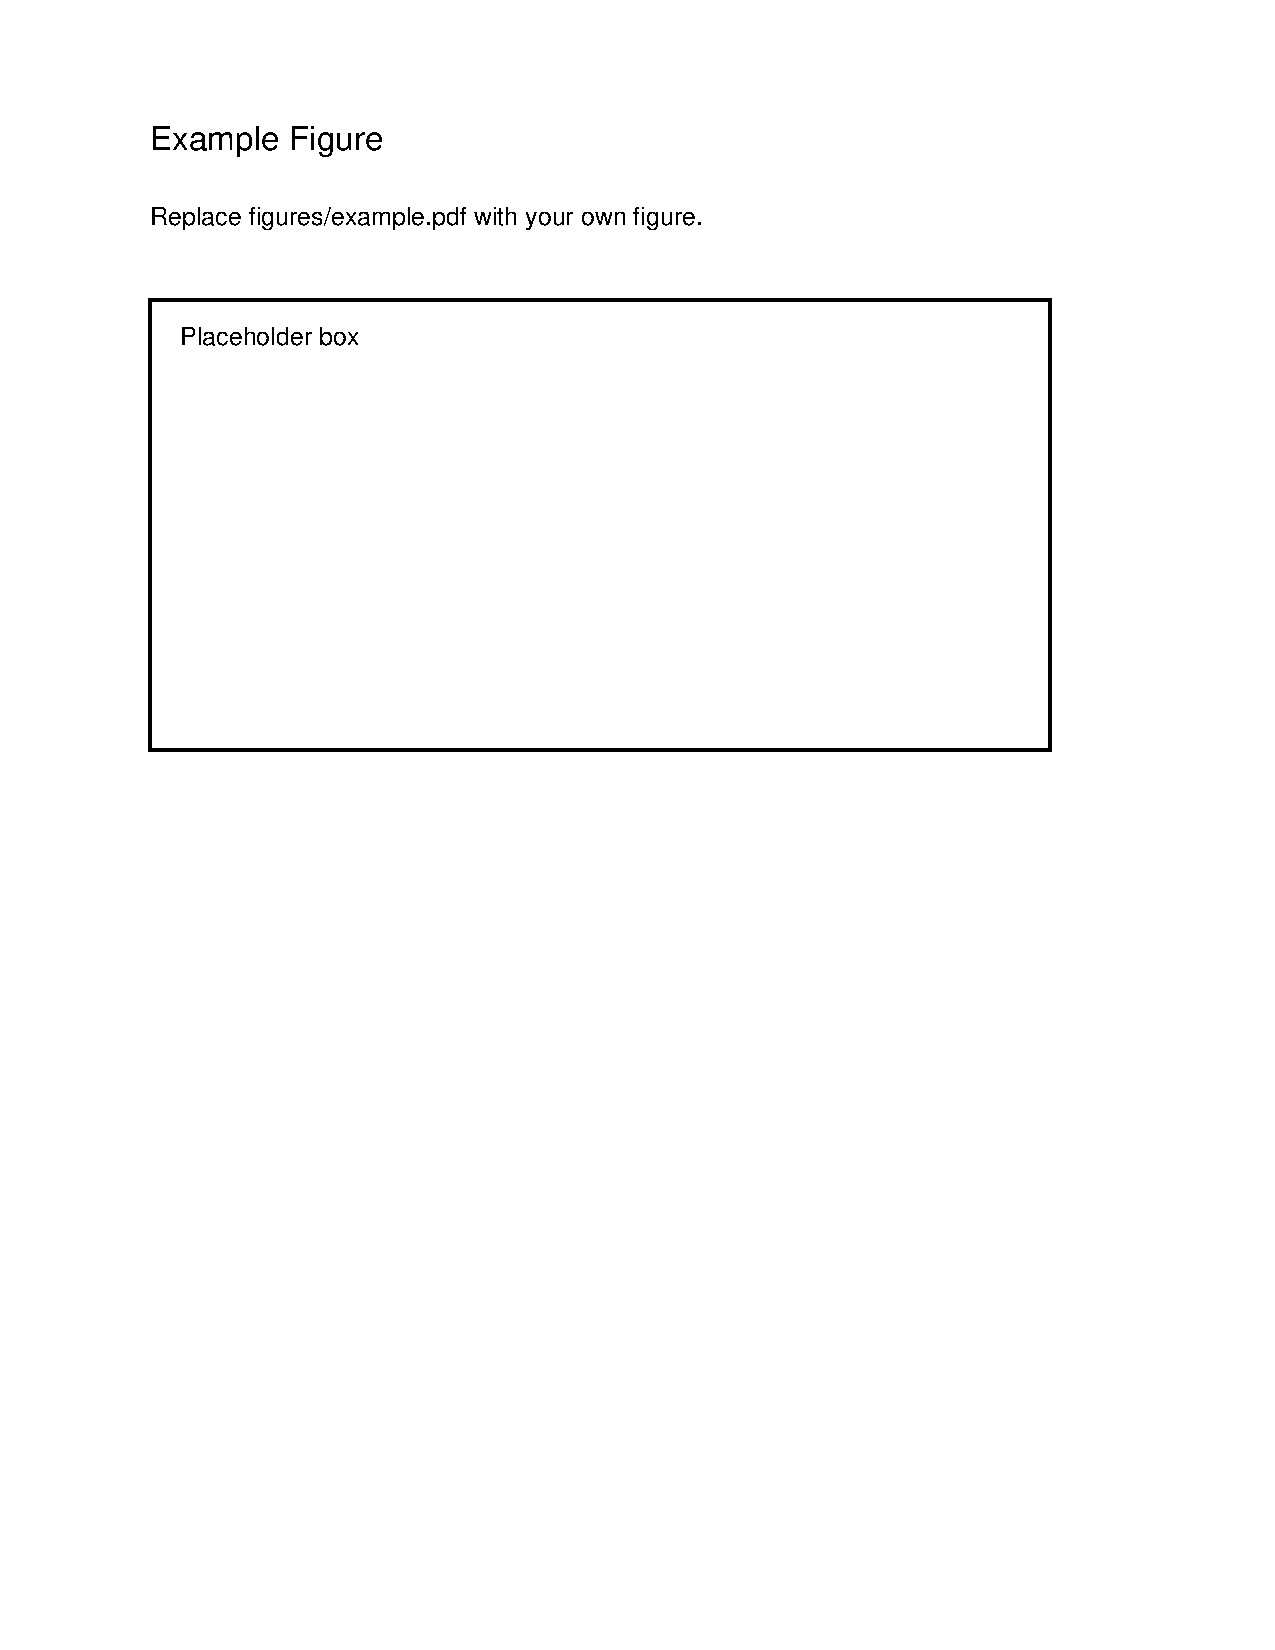
\includegraphics[width=0.45\linewidth]{figures/example.jpg}
  \end{center}
  \caption{多组图示例}
  \label{fig:aa}
\end{figure}

\begin{figure}[htbp]
  \centering
  \begin{subfigure}{\linewidth}
    \centering
    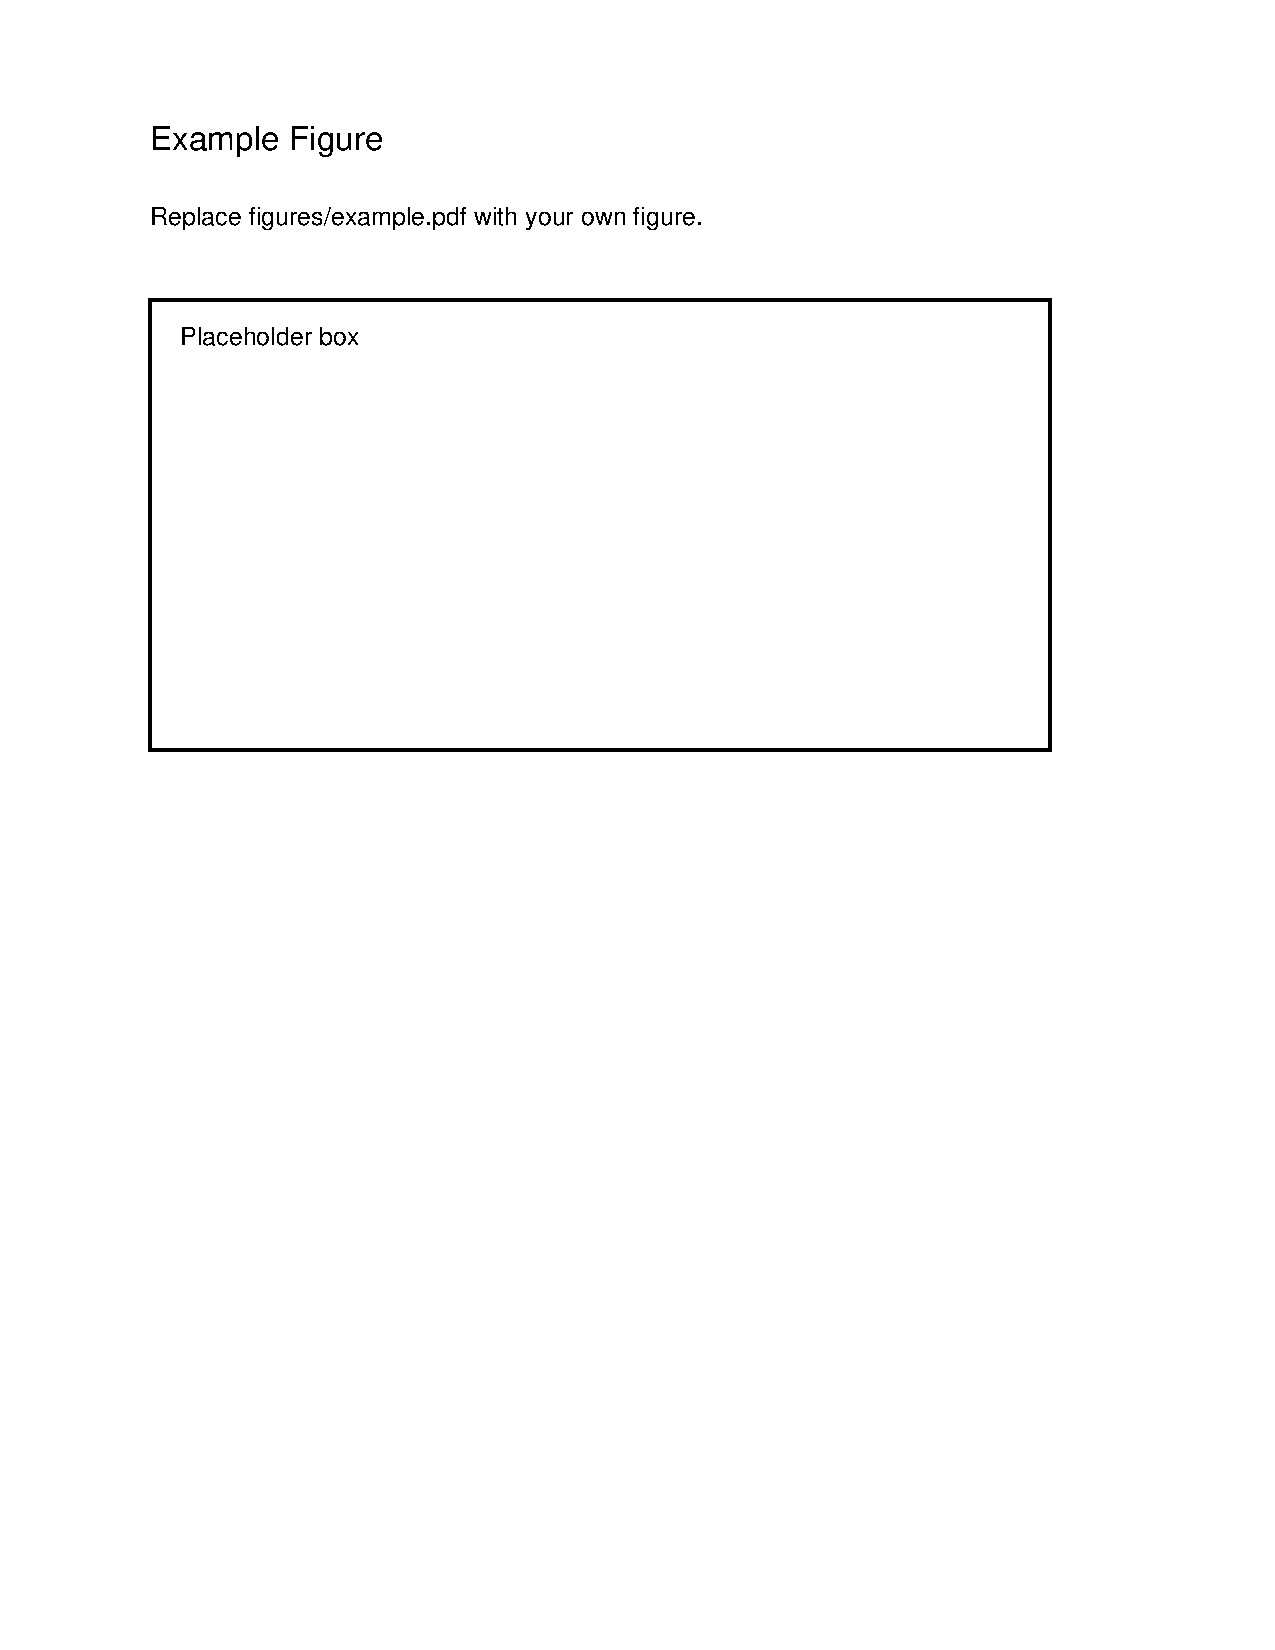
\includegraphics[width=0.45\linewidth]{figures/example.jpg}
    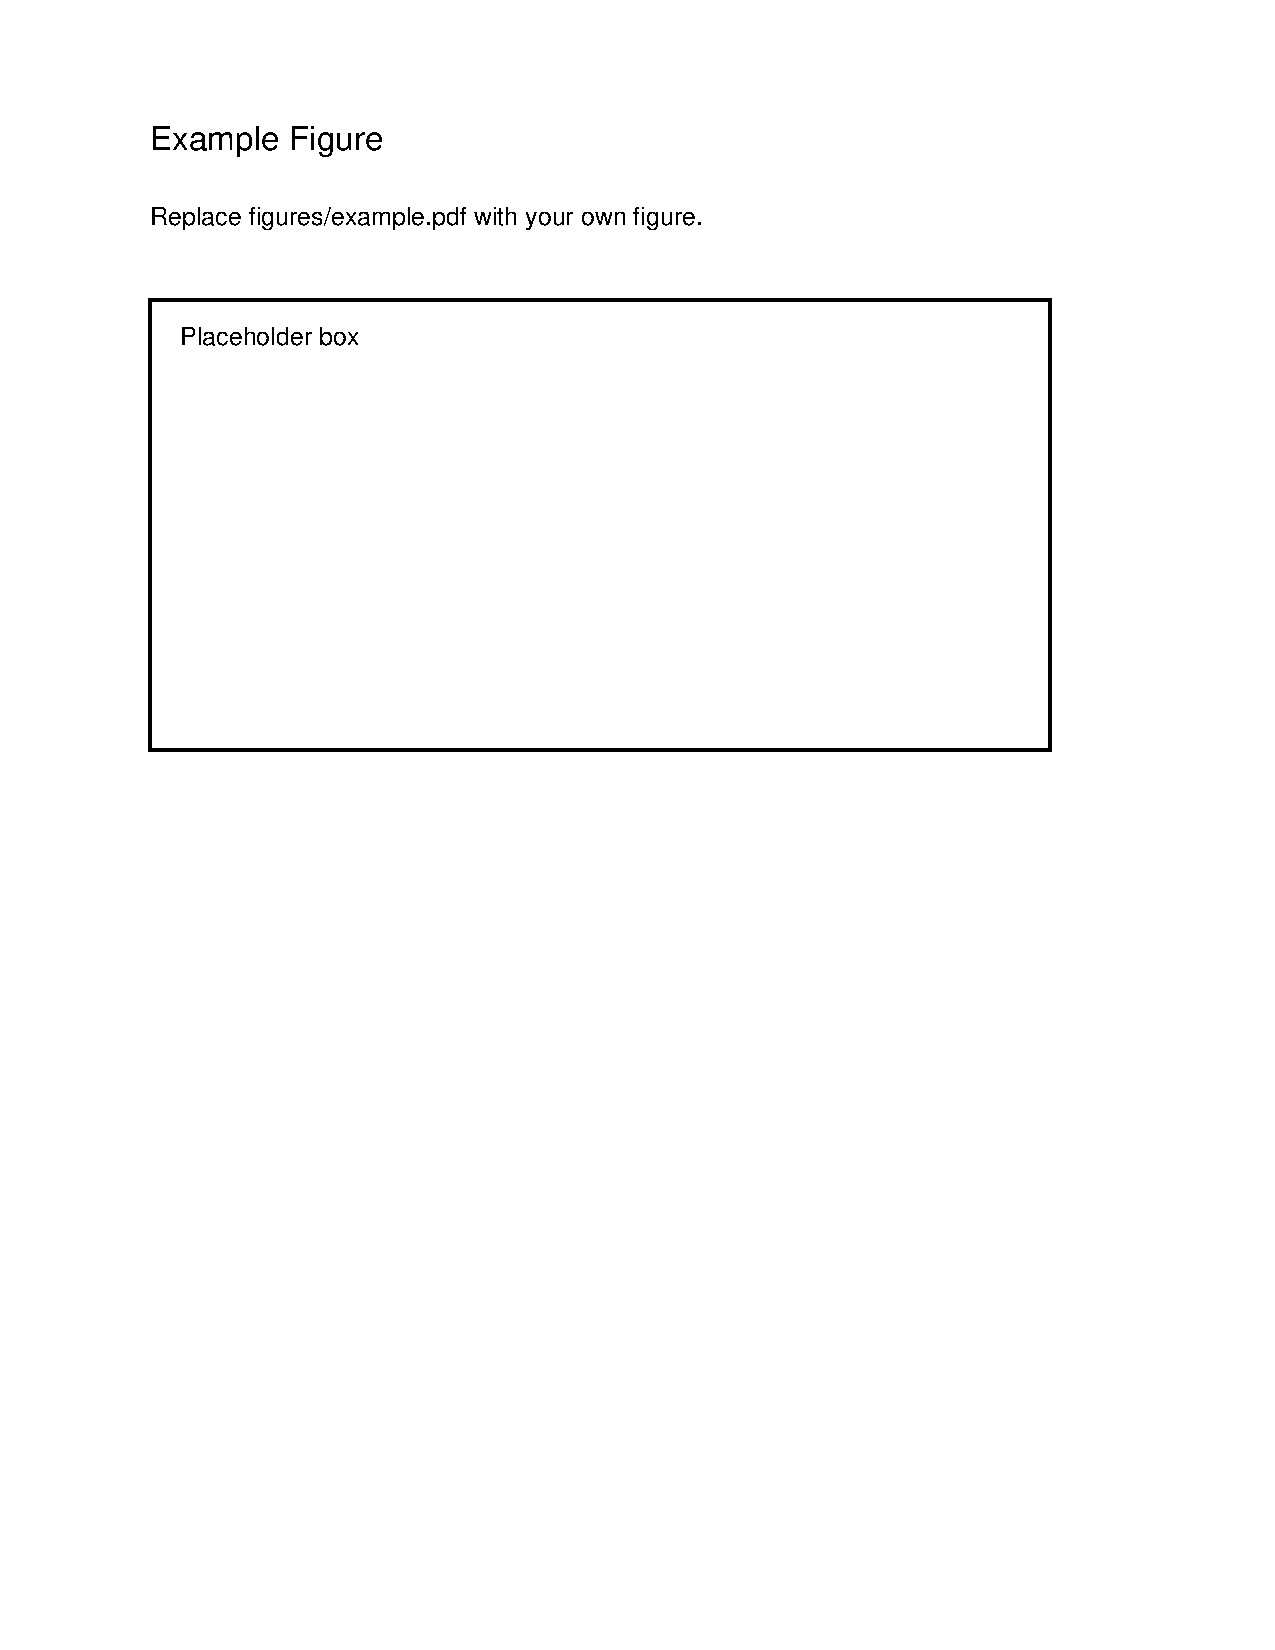
\includegraphics[width=0.45\linewidth]{figures/example.jpg}
    \caption{结果 A}
    \label{fig:a}
  \end{subfigure}
  \hfill
  \begin{subfigure}{0.45\linewidth}
    \centering
    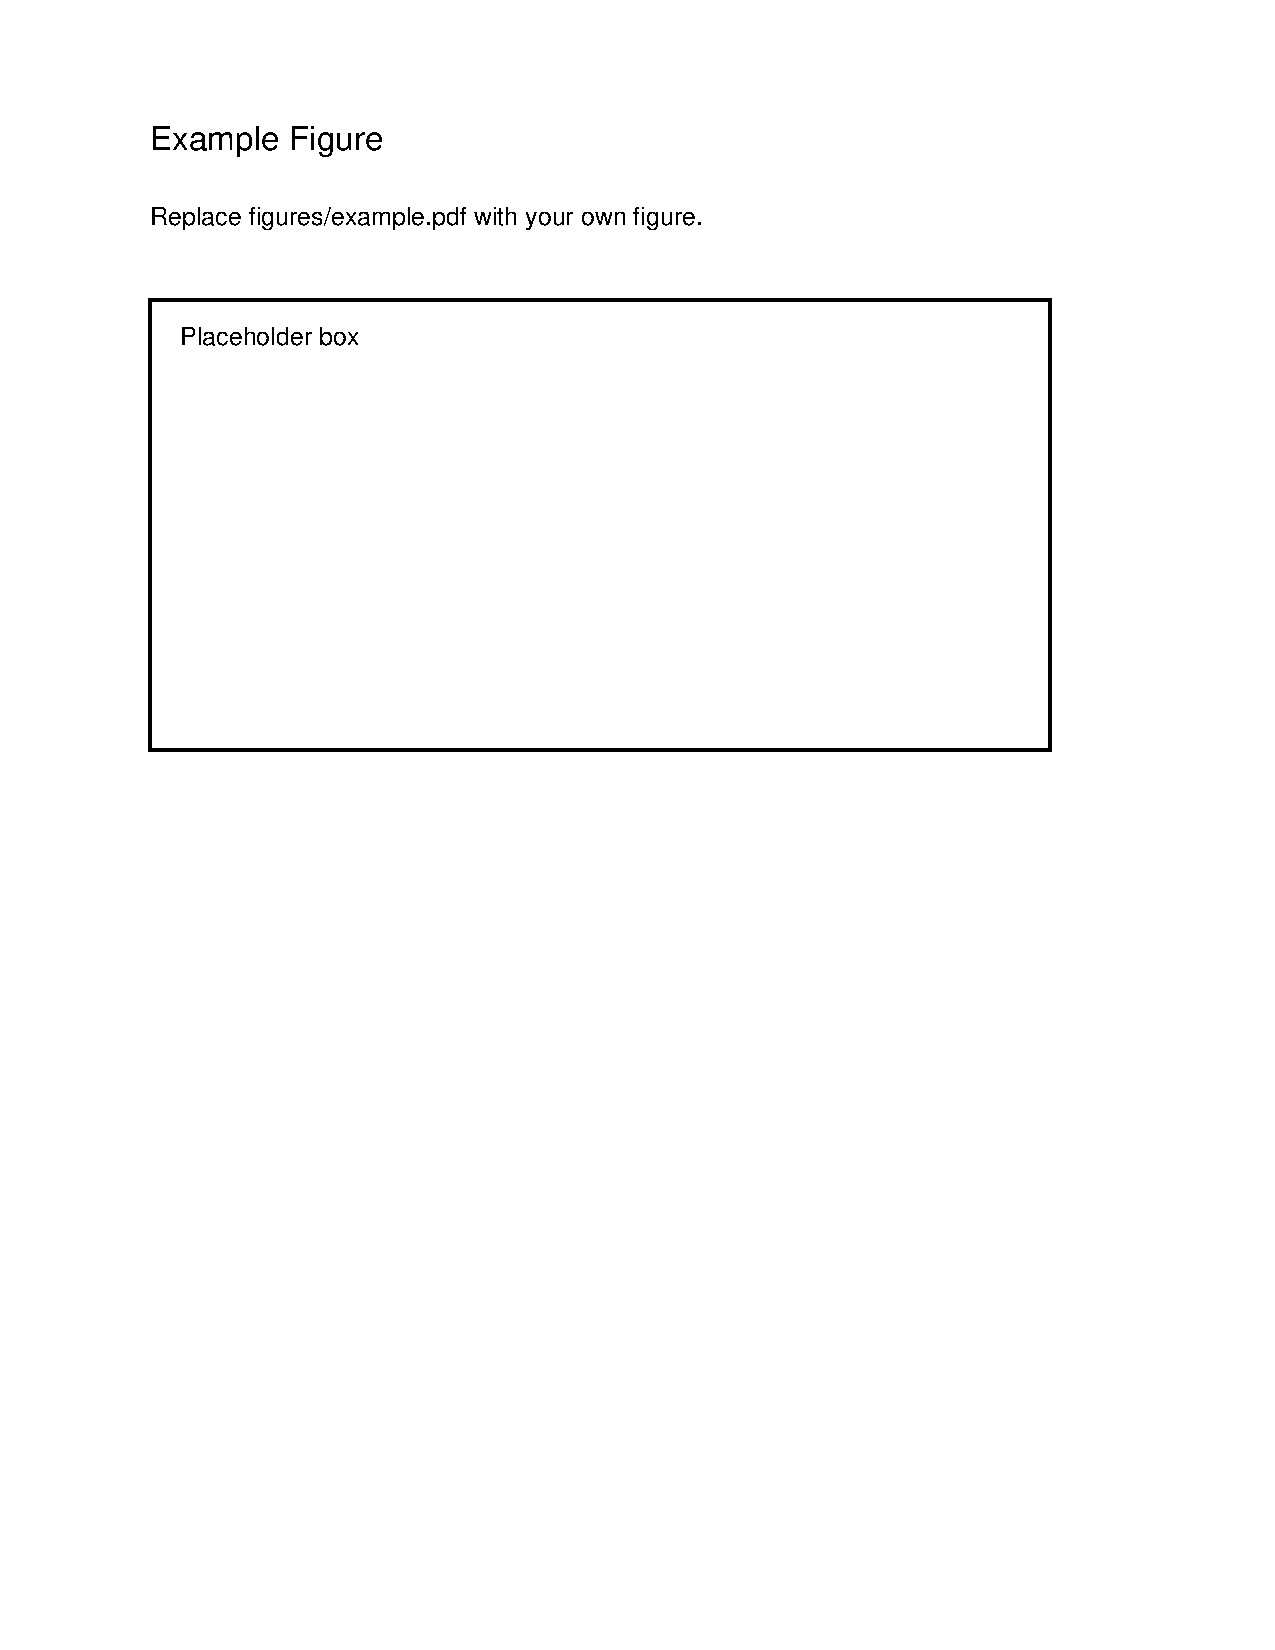
\includegraphics[width=\linewidth]{figures/example.jpg}
    \caption{结果 B}
    \label{fig:b}
  \end{subfigure}
  \caption{不同方法结果对比}
  \label{fig:ab}
\end{figure}



图题应简洁准确,能够独立说明图像内容;所有图形均应在正文中被引用后再出现。

\subsection{一般表格}

表格常用于展示实验数据、参数设置或结果对比。本模板推荐使用三线表格式排版,以增强表格的可读性和规范性。表题位于表格上方,内容示例如下:

\setlength{\tabcolsep}{20pt}
\begin{table}[htbp]
\centering
\caption{不同算法性能比较}
\label{tab:performance}
    \begin{tabular}{lccc}
    \toprule
        算法 & 准确率(\%) & 召回率(\%) & F1 值 \\ 
        \midrule
        算法 A & 92.3 & 90.1 & 91.2 \\
        算法 B & 89.7 & 88.4 & 89.0 \\
        算法 C & 94.5 & 93.2 & 93.8 \\
    \bottomrule
    \end{tabular}
\end{table}

表格中的数据应与正文分析相对应,避免仅罗列数据而缺乏说明。
\subsection{纵向表格}
纵向表格如\cref{tab:wide}所示
\begin{sidewaystable}[p]
\centering
\caption{各算法在不同数据集上的性能对比}
\label{tab:wide}
\begin{tabular}{lcccccccc}
\toprule
方法 & 指标1 & 指标2 & 指标3 & 指标4 & 指标5 & 指标6 & 指标7 & 指标8 \\
\midrule
算法A &  &  &  &  &  &  &  &  \\
算法B &  &  &  &  &  &  &  &  \\
\bottomrule
\end{tabular}
\end{sidewaystable}

\subsubsection{表格合并单元格}
表格合并单元格如\cref{tab:2-3}所示
\begin{table}[ht]
    \centering
    \caption{table:2-3}
    \label{tab:2-3}
    \begin{tabular}{llccc}
    \toprule
    \multirow{2}{*}{数据集}
    & \multirow{2}{*}{方法}
    & \multicolumn{3}{c}{指标} \\
    \cmidrule(lr){3-5}
    & & Acc & Recall & F1 \\
    \midrule
    a & a & a & a & a\\  % 每行后面都要加换行符号
    \bottomrule
    \end{tabular}

\end{table}


\section{算法}

当论文中涉及计算流程或方法步骤时,可使用算法环境进行描述。本模板支持算法自动编号与行号显示,便于表述复杂流程。

算法示例如下:

\begin{algorithm}[H]
    \caption{示例算法}
    \begin{algorithmic}[1]
        \Require 数据集 $D$
        \Ensure 模型参数 $\theta$
        \State 初始化 $\theta$
        \For{$i=1$ to $T$}
            \State 更新 $\theta$
        \EndFor
        \While{$i \le T$}
            \State While 循环
        \EndWhile
    \end{algorithmic}
\end{algorithm}

其中,\texttt{\textbackslash Require} 与 \texttt{\textbackslash Ensure} 分别用于说明算法的输入条件与输出结果。

\section{定理与证明}

对于重要的理论结论、性质或推导结果,可使用定理(Theorem)环境进行表述。模板中定理内容采用斜体排版,以突出其理论性质。

\begin{theorem}[示例定理]
若……则……
\end{theorem}

定理环境同样支持可选标题,用于对定理内容进行简要概括。

定理与证明是理论分析的重要组成部分。定理环境用于陈述结论,证明环境用于给出推导过程。模板中证明环境的“证明.”二字自动加粗,证明内容采用正体排版,格式统一。

\begin{theorem}
    \label{th:1}
    asdasd
\end{theorem}

\begin{proof}
    dsas
\end{proof}

作者在书写证明时,无需额外添加格式命令,仅需关注逻辑推导过程。

\section{引用}

论文中涉及的文献应统一通过 Bib\TeX{} 管理,并在正文中使用引用命令进行标注。例如:

文献引用示例:\cite{example2024paper}

对于定理、公式等对象,建议使用交叉引用方式进行说明:

定理引用方式一:\cref{th:1},方式二:\ref{th:1}。

对于不需要编号的公式,可使用无编号公式环境:

\begin{equation*}
    a = b
\end{equation*}

需要编号的公式使用如下形式:

\begin{equation}
    \label{eq:2}
    a = b
\end{equation}

公式引用方式一:\ref{eq:2},方式二:\cref{eq:2}。

\section{插入代码}

\begin{lstlisting}[language=Java, caption={MapReduce 主流程}, label={lst:mr}]
public static void main(String[] args) {
    System.out.println("Hello, Hist!");
}
\end{lstlisting}



